\chapter{WaveStitch: Flexible and Fast Conditional Time Series Generation with Diffusion Models}

\section{Introduction}
As I mentioned, \textbf{Wavestitch} is the diffusion model I have been tasked with researching.  
In this chapter, I would like to provide a general overview of it using the paper that describes it.  
The document begins by showing the three critical issues identified by the authors in the conditional generation of time series—the lack of adaptability of existing models to inference conditions, the slowness of autoregressive generative processes, and inefficiency in the encoding of categorical characteristics—which have been addressed through innovative and efficient solutions: a flexible conditioning mechanism, a parallel generation procedure with segment \emph{stitching}, and cyclic encoding of categorical variables.  
These methodological choices make it possible to overcome the structural limitations of previous models, leading to significant improvements in both accuracy and computational efficiency~\cite{wavestitch} .

\section{Challenges addressed}

\subsection{Q1: Adaptability to inference conditions}S
One of the most significant limitations of existing generative models is their poor ability to adapt to changing conditions during inference.  
In many application contexts, time series depend not only on their historical trends, but also on auxiliary variables or metadata (e.g., year, month, district, type of service).  
Models such as TimeGAN or conditioned LSTM variants are trained on fixed configurations of conditions, which limits their ability to generalize to scenarios never seen during training.  
This rigidity translates into low operational flexibility: if new combinations are required during inference (e.g., a specific year associated with a brand not present in the training), the models are unable to adapt and produce inconsistent or statistically implausible samples~\cite{yoon2019timegan}.

\subsection{Q2: Slowness of autoregressive methods}
Most classical methods for generating time series are \emph{autoregressive} in nature, i.e., they generate values one at a time, using sliding windows.  
While this approach ensures sequential consistency, it comes at a very high computational cost: generation becomes slow and difficult to parallelize, especially when working with large datasets or extended time horizons.  
For real-world applications—such as monitoring energy consumption in an HPC center or managing healthcare data—speed is a fundamental requirement.  
A method that takes minutes or hours to generate a synthetic sequence is impractical, especially when integrated into simulation or \emph{real-time decision-making} systems.  
Consequently, the slowness of sequential methods represents a real obstacle to their industrial adoption~\cite{yoon2019timegan,zhou2023timeweaver}.

\subsection{Q3: Inefficient encoding of categorical features}
Time series are often influenced by categorical features, such as days of the week, months, or codes indicating membership in a certain group of devices.  
The most commonly used method for representing these variables is \emph{one-hot encoding}, which, however, has two main limitations:
\begin{itemize}
    \item it significantly increases the dimensionality of the input, making the model heavier and more difficult to train;
    \item it does not naturally represent the periodicity of variables, such as daily or monthly cycles, where extreme values (e.g., December and January) should be close together but are instead placed at opposite ends of the coding spectrum.
\end{itemize}
This inefficiency in representation results in a loss of structural information, which can compromise the model’s ability to capture cyclical regularities typical of energy, financial, or environmental time series.  
These challenges constitute the motivational context within which WaveStitch was developed, whose architecture aims to provide innovative solutions for each of the problems highlighted~\cite{wavestitch}.

\section{Methodology and proposed solution}

The methodology behind \textbf{WaveStitch} stems from the need to systematically address the three main challenges identified in the previous paragraph.  
The authors propose an architecture that exploits \emph{Denoising Diffusion Probabilistic Models} (DDPMs)~\cite{ho2020ddpm}.

\subsection{Flexible constraint management (Q1)}
The first innovation of WaveStitch concerns its ability to generalize to conditions never seen during training.  
The model is trained in two distinct phases:
\begin{enumerate}
    \item \textbf{Training:} the denoiser is trained to generate a complete signal conditioned \emph{only} on auxiliary characteristics (e.g., year, month, region).  
    \item \textbf{Inference:} at the time of generation, constraints from the actual values of the observed signal (e.g., available portions of the series) are also introduced.  
    Through conditional masks, the model integrates this partial information and produces coherent sequences that comply with both metadata and historical data.  
\end{enumerate}
This approach makes WaveStitch flexible and capable of adapting to unexpected scenarios, such as the request to generate a time series block for combinations of conditions not present in the training dataset~\cite{wavestitch}.

\subsection{Parallel generation with stitching (Q2)}
To solve the problem of slow autoregressive methods, the authors introduce a \textbf{parallel generation} mechanism.  
The signal and conditions are divided into overlapping windows, processed in parallel by mini-batches.  
After each denoising step, the overlapping portions are reconciled through a \emph{stitching} process, which consists of overwriting the common regions with the values generated by the previous window.  

\begin{itemize}
    \item This process maintains sequential consistency between independent segments.  
    \item The computational complexity is reduced from $O(T \cdot t_\theta(w) \cdot (M-w)/s)$ (autoregressive) to $O(T \cdot t_\theta(w) \cdot (M-w)/(b \cdot s))$, where $b$ is the batch size.  
    \item In practice, this translates into a \textbf{speedup of up to 460 times} compared to sequential methods, without sacrificing the quality of the synthetic signal.  
\end{itemize}

This solution combines the speed of parallel generation with temporal consistency, which until now has been the prerogative of autoregressive models.  
The mechanism is shown in Figure~\ref{fig:stitching_paper}, which illustrates the parallel generation flow: overlapping windows are processed by multiple denoisers in parallel and then integrated through the \emph{stitching} process in common regions~\cite{wavestitch}.

\begin{figure}[H]
\centering
    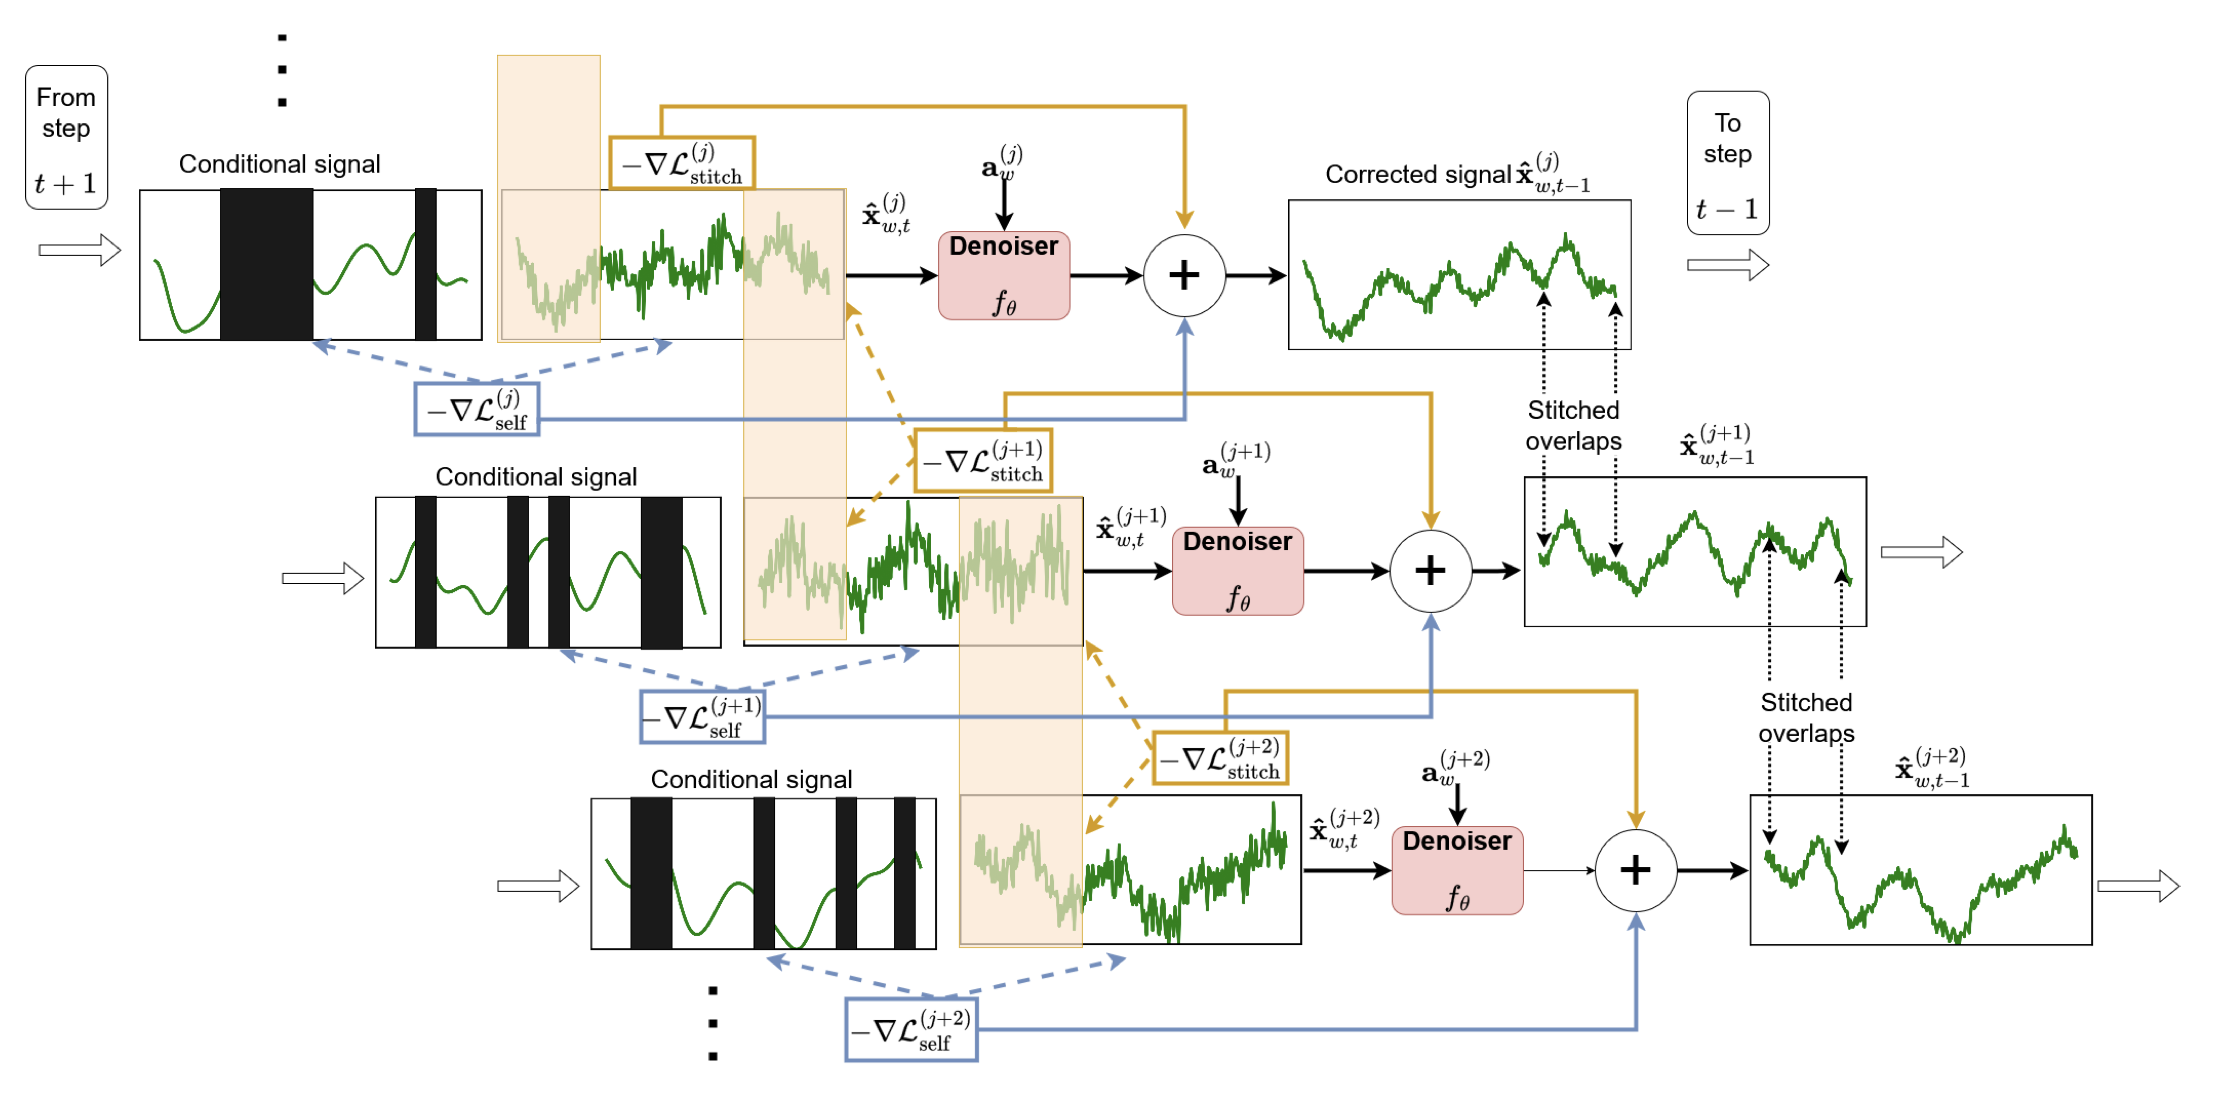
\includegraphics[width=\textwidth]{images/stitchComplex.png}
    \caption{\emph{Stitching} mechanism in WaveStitch: overlapping windows are denoised in parallel and reconciled in common areas to maintain sequential consistency. (Adapted from \cite{wavestitch}).}
    \label{fig:stitching_paper}
\end{figure}

\subsection{Cyclic encoding of categorical variables (Q3)}
The third innovation in WaveStitch concerns the representation of categorical features.  
Instead of using traditional \emph{one-hot encoding}, the authors propose a \textbf{cyclic encoding}:

\[
\theta_k = \frac{2\pi k}{K}, \quad
\text{with } k = 0,1,\dots,K-1
\]
\[
a_{sin}(k) = \sin(\theta_k), \quad a_{cos}(k) = \cos(\theta_k)
\]

Each categorical variable is then mapped to two coordinates $(\sin, \cos)$ on a unit circle.  
This approach has three main advantages:  
\begin{itemize}
    \item it drastically reduces dimensionality (from $K$ to 2 dimensions);  
    \item it preserves the cyclical nature of the variables (for example, December and January are close on the circumference, unlike what happens with one-hot encoding);  
    \item it decreases the sparsity of the input, making training more efficient~\cite{wavestitch}.  
\end{itemize}

\section{Experiments and results}

To validate the proposed approach, the authors of \textbf{WaveStitch} conducted a series of experiments on public datasets from different domains:  
\emph{Beijing Air Quality}, \emph{Metro Traffic Volume}, \emph{Panama Energy}, \emph{Rossman Sales}, and \emph{Australia Tourism}.  
These datasets include univariate and multivariate signals, including both continuous variables (e.g., energy consumption, traffic volume) and categorical features (e.g., year, month, district)~\cite{wavestitch}.

\subsection{Experimental setup}
\begin{itemize}
    \item \textbf{Hardware configuration:} The experiments were performed on an AMD Ryzen 9 5900 processor with 12 cores and an NVIDIA RTX 3090 GPU, demonstrating the need for substantial computing resources for training diffusion models.  

    \item \textbf{Data division:} The test sets were constructed to contain combinations of completely new auxiliary conditions, such as a year that was never present in the training set.  
    This made the evaluation more realistic and rigorous.  

    \item \textbf{Tasks evaluated:} imputation of missing values, short-term forecasting, and generation of synthetic scenarios under multi-level constraints (\emph{Root}, \emph{Intermediate}, \emph{Bottom}).  

    \item \textbf{Metrics:} The authors adopted a mix of point and structural metrics:  
    \begin{itemize}
        \item \emph{Mean Squared Error (MSE)} to quantify numerical accuracy;  
        \item \emph{Autocorrelation Difference (ACD)} to measure similarity in temporal patterns;  
        \item \emph{Cross-feature Correlations (x-Corr)} to evaluate dependencies between multivariate variables~\cite{wavestitch}.  
    \end{itemize}
\end{itemize}

\subsection{Main results}
The experimental results clearly show the advantages of WaveStitch:  
\begin{itemize}
    \item in terms of MSE, the model achieves up to \textbf{10 times better performance} than the baselines (e.g., TSDiff, TimeWeaver, TimeGAN), particularly in the \emph{Australia Tourism (B)} task;  

    \item the stitching mechanism allows for \textbf{460 times faster} generation than the traditional autoregressive approach, while maintaining comparable MSE values;  

    \item in structural metrics, WaveStitch better preserves autocorrelations and cross-correlations, demonstrating that it replicates not only point values but also deep statistical relationships in the data~\cite{wavestitch,tashiro2021csdi,zhou2023timeweaver,yoon2019timegan}.  
\end{itemize}

\subsection{Comparative table}
An excerpt of the results reported by the authors is shown in Table~\ref{tab:wave-results}, which summarizes the performance of WaveStitch compared to the most relevant baselines.  

\begin{table}[H]
\centering
\setlength{\tabcolsep}{10pt}
\renewcommand{\arraystretch}{1.15}
\begin{tabular}{| l | l | c | c | c |}
\hline
\rowcolor[HTML]{F87C58}
\textbf{Dataset / Task} & \textbf{Method} & \textbf{MSE} & \textbf{ACD} & \textbf{x-Corr} \\
\hline
AustraliaTourism (B) & TimeGAN~\cite{yoon2019timegan}    & 1.580 & 0.231 & 0.298 \\ \hline
                     & TSDiff/CSDI~\cite{tashiro2021csdi} & 1.420 & 0.185 & 0.271 \\ \hline
\rowcolor[HTML]{FDE5DC}
                     & WaveStitch~\cite{wavestitch}       & \textbf{0.153} & \textbf{0.072} & \textbf{0.101} \\ \hline
MetroTraffic (I)     & TimeWeaver~\cite{zhou2023timeweaver} & 0.864 & 0.210 & 0.322 \\ \hline
                     & TSDiff/CSDI~\cite{tashiro2021csdi}   & 0.701 & 0.175 & 0.285 \\ \hline
\rowcolor[HTML]{FDE5DC}
                     & WaveStitch~\cite{wavestitch}          & \textbf{0.312} & \textbf{0.090} & \textbf{0.133} \\ \hline
\end{tabular}
\caption{Comparison of methods: MSE (error), ACD (autocorrelation difference), x-Corr (correlation difference).  
The values show WaveStitch’s ability to reduce numerical error (MSE) and preserve statistical structures (ACD, x-Corr); values adapted from \cite{wavestitch}.}
\label{tab:wave-results}
\end{table}

\section{Connection to this work}

Perfect, now we know why the techniques introduced by WaveStitch can be directly applied to my work.  
Following the approach of the authors, who validated the model on benchmark datasets such as \emph{Metro Traffic} and \emph{Australia Tourism}, as I mentioned in the previous chapter, I chose to replicate the analysis, training, and evaluation flow by applying it to real energy data from the HPC center in Turin.  
In particular, the core of my work is the concepts of imputation, synthetic scenario generation, and conditional forecasting, which I will show how I have adapted to the context of monitoring rack consumption and electrical variables, with the aim of verifying the validity of the model in a complex and noisy environment.